\section{ASCII}
\subsection{Definisi ASCII}
		Berdasarkan artikel yang ditulis oleh hieronymus \cite{hieronymus1993ascii}
	ASCII atau American Standard Code for Information Interchange merupakan sebuah pengkodean berstandar Internasional yang berupa kode huruf dan simbol, seperti Hex dan Unicode dan juga merupakan simbol tambahan dari database. ASCII bersifat universal contohnya 124 untuk karakter "|". ASCII selalu digunakan oleh komputer dan alat komunikasi yang lain untuk menunjukkan teks.
    Dalam kode ASCII mempunyai komponen komponen bilangan biner yang berjumlah 7 bit. Kode ASCII berfungsi untuk mewakili karakter angka ataupun huruf di dalam komputer. Sebuah pengkodean ASCII dari Afabet Fonetik Internasional atau IPA dirancang untuk semua bahasa. Skema ASCII yang akan dibuat serupa dengan simbol IPA dasar sehingga akan banyak simbol yang memiliki makna jelas dan banyak simbol yang sama dengan skema yang lain. Prinsip dasarnya merupakan spectrally dan tempor berbeda yang memiliki sifat fonemik.
    Dalam beberapa bahasa harus memiliki simbol dasar yang terpisah. Dalam kebanyakan kasus, simbol dasar terdiri dari aconcatenation dari simbol IPA. Dengan demikian mudah untuk mengenali simbol dasar fonemik dan membandingkan suara fonetik lebar yang sama di seluruh bahasa. Bahasa nada telah diacritics dan diterapkan pada simbol fonem vokal untuk mengidentifikasi fonem dengan benar dalam bahasa-bahasa ini. Allophonic variasi karena koartikulasi dan stress kontek stual dapat diberi label.
	Simbol dasar Ada kemungkinan bahwa beberapa suara ucapan yang merupakan fonemiK.Satu dar iyang lain hilang dari versi sekarang. Diharapkan setiap kelalaian akan terjadi dikoreksi dalam versi Worldbet berikutnya, dan menggunakan metode standar untuk membangun simbol yang baru. Alfabet Fonetik Internasional dikembangkan di Indonesia pada tahun 1888 dan ada beberapa kali revisi kedalam bentuknya yang sekarang. Ini mewakili 105 tahun pengalaman dengan meletakkan simbol untuk setiap suara dalam semua bahasa yang dikenal di dunia.
	Representasi dan perbedaan antara variasi alofonik dan suara base form sejati telah terjadi
	bekerja untuk lebih banyak bahasa sejak IPA diformulasikan.
	tempat untuk memulai untuk multi bahasa pidato database pelabelan eortort.
	Ada beberapa suara yang biasanya tidak termasuk dalam IPA yang telah ditemukan
	berguna untuk memberi label pada corpora ucapan besar seperti TIMIT, SCRIBE, BDSON, dan PHONDAT. Ini
	Upaya modern mengenai bentuk standar ASCII IPA menghasilkan TIMITBET, MRPA, SAMPA, dan
	SAMPA Diperpanjang untuk beberapa nama dari mereka. Huruf fonetik ini dibatasi untuk bahasa Inggris atau bahasa Inggris kebahasa-bahasa Eropa.
	ASCII memiliki jumlah kode sebanyak 255 dengan nilai ANSI ASCII desimal 0 sampai 127 merupakan kode ASCII manipulasi teks sedangkan kode ASCII dengan nilai ANSI ASCII 128 sampai 255 merupakan kode ASCII untuk memanipulasi gambar grafik.
	\begin{enumerate}
		\item Kode yang tidak terlihat seperti kode 8 back space,10 pergantian baris,32 spasi
		\item sedangkan kode yang terlihat simbolnya seperti numerik atau angka 0...9 abjad a...z karakter khusus.
		\item dan kode yang tidak ada di keyboard tapi tidak dapat ditampilkan, kode-kode ini biasanya untuk kode-kode grafik dengan nilai ANSI ASCII 128 sampai 225.
  \end{enumerate}

	Berikut contoh tabel berisi karakterk-karakter ASCII.
\begin{table}[H]
\begin{tabular}{|c|c|c|c|c|}
hline
Karakter & Nilai Unicode (heksadesimal) & Nlai ANSI ASCII(desimal) & Keterangan\\
\hline
NUL & 0000 & 0 & Null(tidak tampak)\\
SOH & 0001 & 1 & Start of Heading(tidak tampak)\\
0 & 0030 & 48 & Angka nol\\
1 & 0031 & 49 & Angka satu\\
2 & 0032 & 50 & Angka dua\\
3 & 0033 & 51 & Angka tiga\\
4 & 0034 & 52 & Angka empat\\
5 & 0035 & 53 & Angka lima\\
6 & 0036 & 54 & Angka enam\\
7 & 0037 & 55 & Angka tujuh\\
8 & 0038 & 56 & Angka delapan\\
9 & 0039 & 57 & Angka sembilan\\
\hline
\end{tabular}
\end{table}

\subsection{Prinsip-Prinsip Umum ASCII}

 Dalam ASCII dikenal juga Worldbet. Worldbet adalah versi ASCII dari  International Phonetic Alphabet (IPA) dengan tambahan luas simbol fonetik yang saat ini tidak ada di IPA. Worldbet ini dirancang untuk sejumlah besar bahasa termasuk Bahasa India, Asia, Afrika dan Eropa. Pertimbangan suara khusus di masing – masing bahasa ini mengarah pada prinsip bahwa setiap simbol dasar akan mewakili suara ucapan urutan waktu yang berbeda secara spektral. Setiap jenis / r / akan memiliki IPA yang terpisah, bukan r graphemic yang digunakan di beberapa label. Allophones seperti plorives aspirated akan memiliki simbol dasar terpisah dari plosives yang tidak diaspirasikan, mereka adalah fonemik dalam bahasa di pertanyaan, jika tidak mereka akan ditandai dengan menggunakan simbol dasar plus (diakritik). Begitu berbeda secara spektral atau temporer karena secara perseptual berbeda, ketika komponennya didengar dalam isolasi. Vokal digolongkan ke posisi posisi nominal. Hal ini diakui bahwa warna vokal rinci dapat bervariasi antara bahasa untuk vokal nominal yang sama, namun simbol yang terpisah hanya akan ditetapkan ketika perbedaan cukup besar untuk membentuk fonem yang berbeda.

 	Dalam pengalaman pelabelan sebenarnya Telah ditemukan bahwa sebagian besar perbedaan dalam label fonetik antara fonetiker terlatih karena ketidaksepakatan pada warna vokal rinci, bukan warna vokal luas sebenarnya. Oleh karena itu, simbol dasar Worldbet akan mewakili perbedaan fonemik dalam beberapa bahasa, seperti pada contoh plosif Simbol dasarnya dimaksudkan untuk menjadi fonetis yang luas, namun dapat digunakan sebagai simbol fonemik permukaan dalam bahasa tertentu (seperti yang dinyatakan dalam asas asli IPA).

 	IPA telah digunakan selama lebih dari 100 tahun dan telah aktif dikembangkan dan berkembang. Selama periode ini, seharusnya semua perbedaan fonemik diamati dalam bahasa dunia saat ini. Oleh karena itu, ini adalah titik awal alami untuk setiap upaya membangun rangkaian fonem yang mana cukup untuk mencakup semua bahasa di dunia.
 	Diacritics digunakan secara umum untuk memodifikasi simbol dasar untuk menangani alofon yang ada karena koartikulasi e-ects (yaitu: labialized / s / di lingkungan / w /), atau konteks fonologis e. Diacritic memungkinkan atrofi tertentu ditandai, yang memiliki karakter dasarnya telepon umum berbasis fonemik yang merupakan asal alofon ini. Tentu saja tidak selalu mudah untuk menentukan variasi alofonik dan apakah perubahan kategori fonetis yang luas. Biasanya jumlah simbol yang akan digunakan untuk memberi label pada bahasa tertentu akan dibatasi, untuk dijaga dari persediaan label yang terlalu besar. Faktor pendorong untuk Worldbet adalah memberi label pidato untuk penelitian ucapan yang didorong oleh korpus, secara fonologis inventaris, identifikasi bahasa otomatis, pengenalan ucapan multi bahasa, dan Multilanguage sintesis ucapan Ini juga berguna dalam membangun kamus multi bahasa. pernyataan ini terdapat dalam artikel yang ditulis oleh cerf. \cite{cerf1969ascii}

    Pada gambar (\ref{fig:ASCII}) adalah gambar dari tabel ASCII.
\begin{figure}[!htbp]
  \centering
  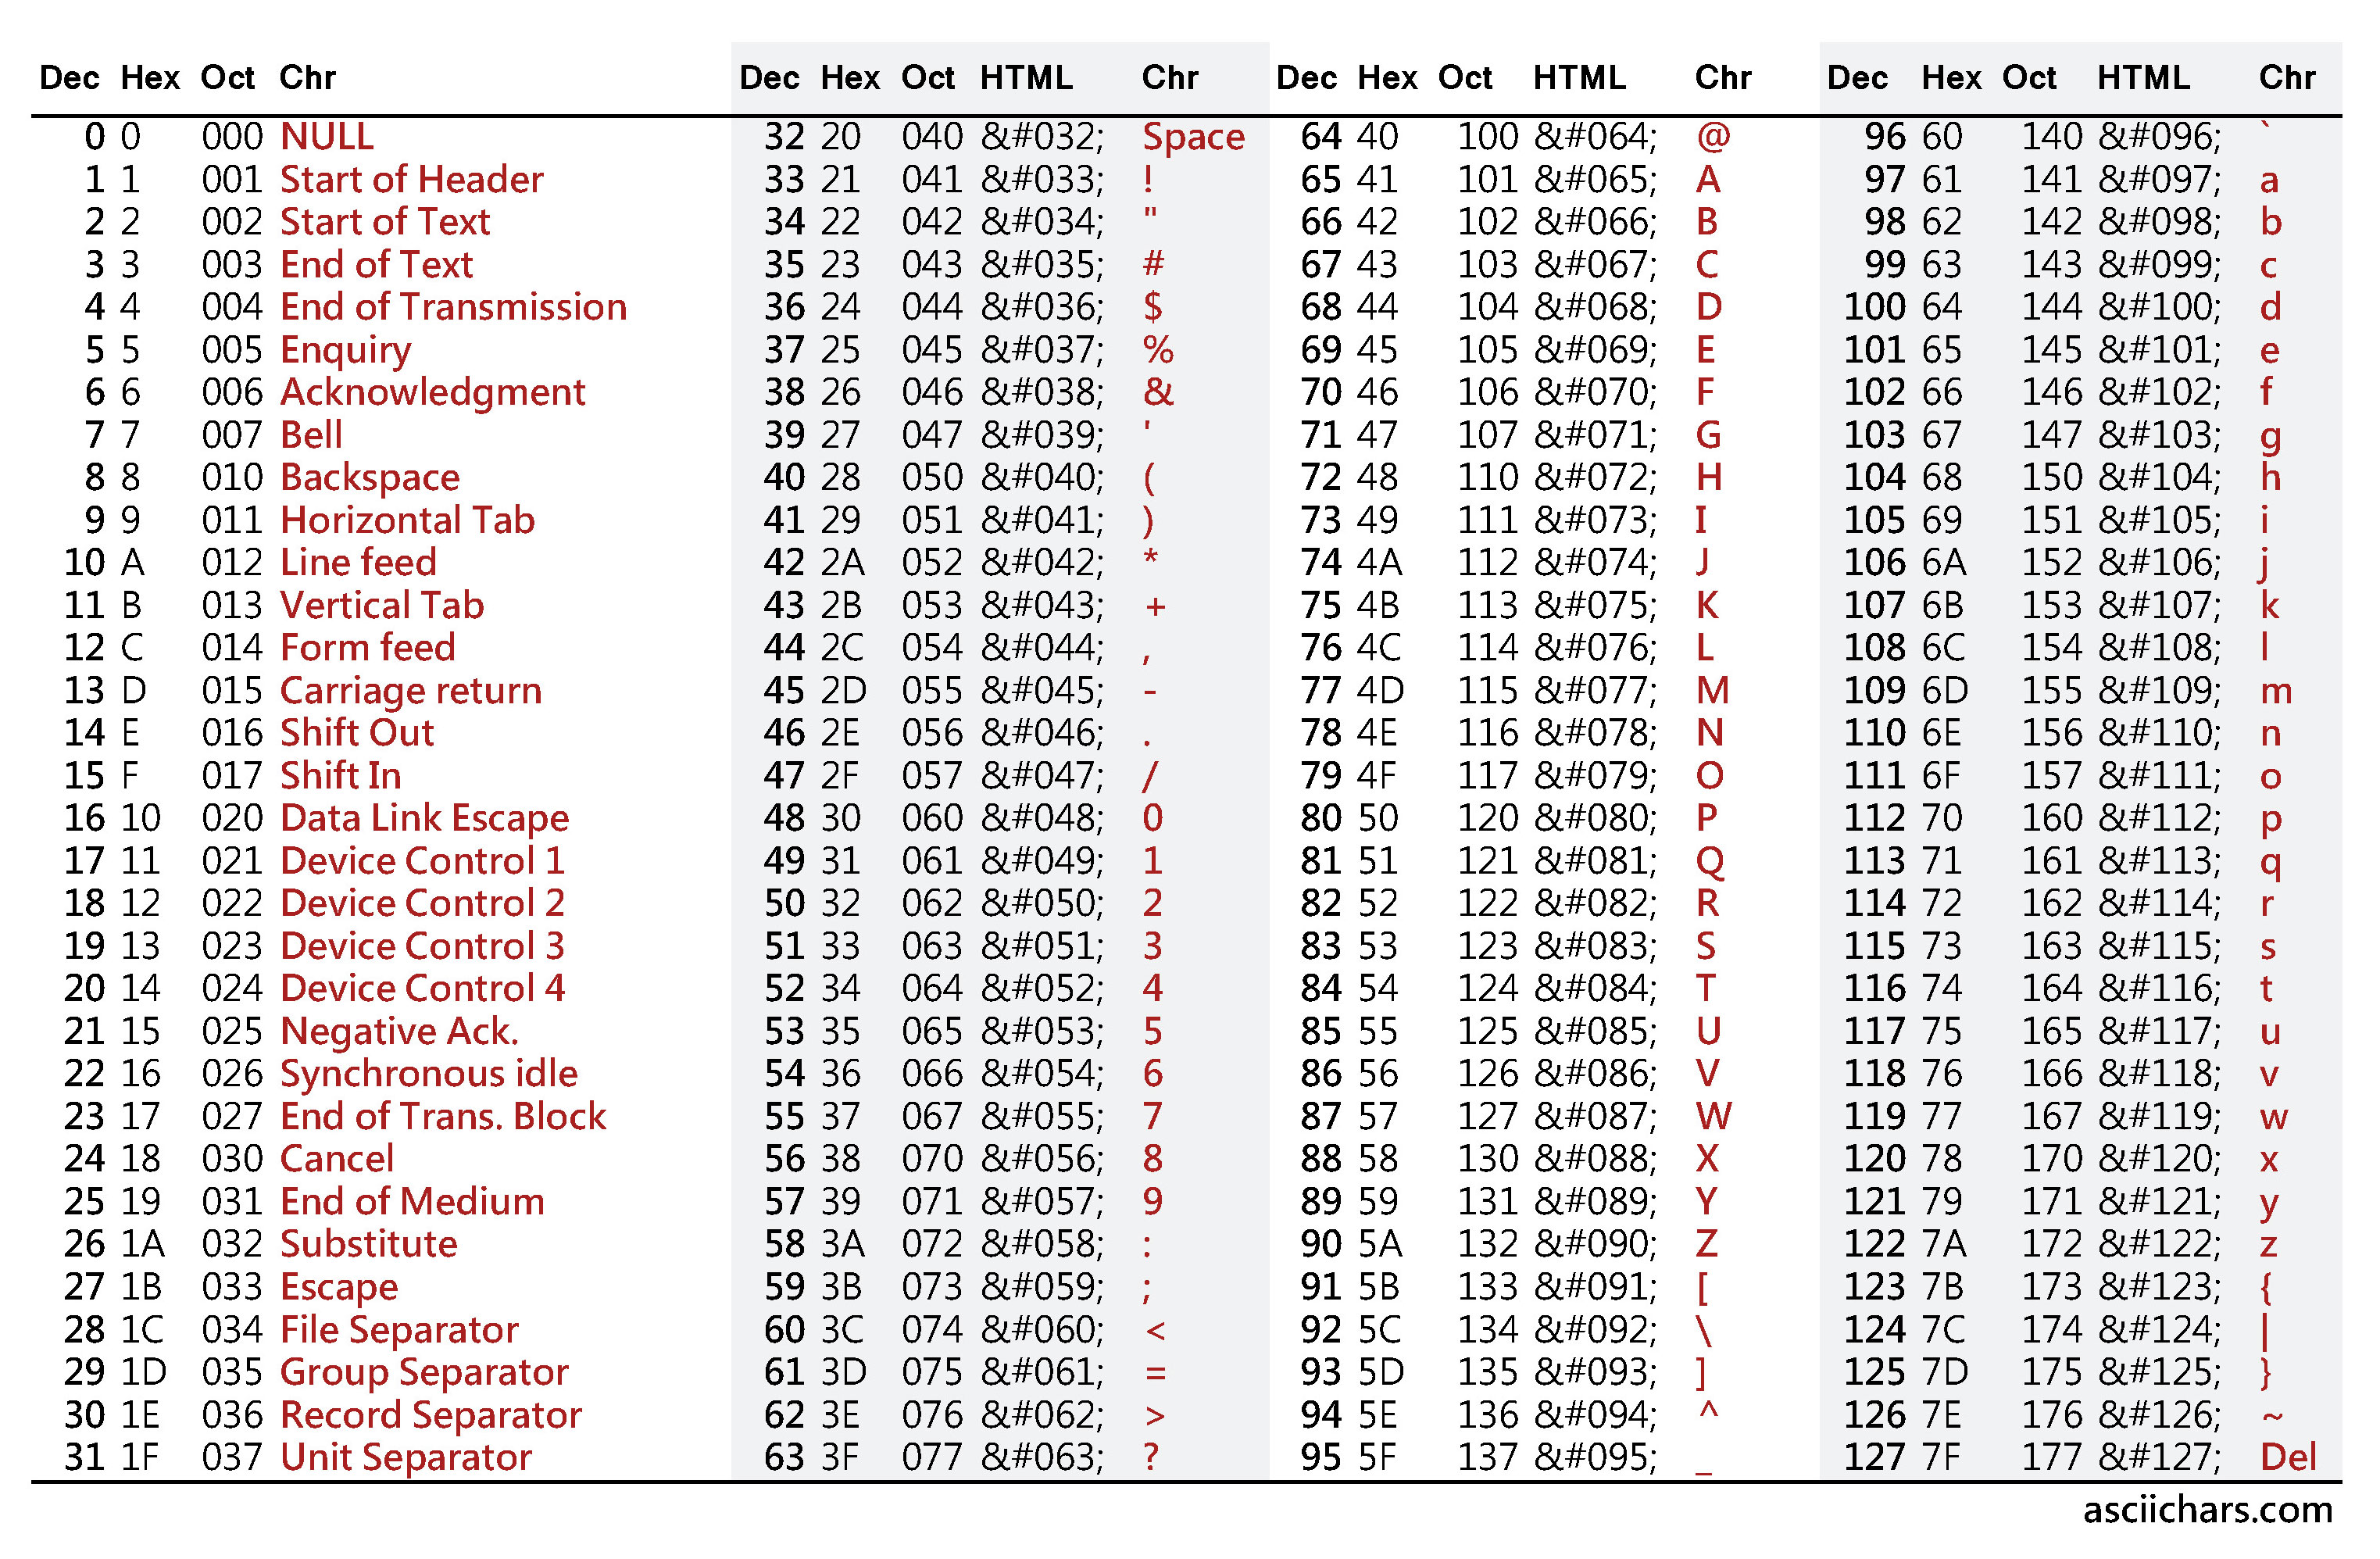
\includegraphics[width=.75\textwidth]{figures/Standar/ASCII.jpg}
  \caption{Ini adalah Gambar dari table ASCII}\label{fig:ASCII}
\end{figure}

\section{UTF-8}
\begin{lstlisting}
\{ \begin{figure}
     \centering
     \includegraphics[width=.75]{}
     \caption{}\label{}
   \end{figure}}
\end{lstlisting} 